\subsection{Checkerboard with Full Coverage}
\label{subsec:checkerboard_results}

Three checkerboards fill a $24\times12\times12$~km domain, with velocities of 4.75 and 5.25~km/s and cube sides of 6, 4, or 3~km ($n_x=4,6,8$). All use 1200 events and 98 surface stations (Figure~\ref{fig:checkerboard_geometry_current}). The forward grid spacing is 125~m, with 1\% relative and 0.01~s absolute pick noise (Section~\ref{subsec:synthetic_data}).

Both start from 5~km/s and use 1-km velocity grids: constant cells for EMTomo and trilinear interpolation for tomoDD. EMTomo uses 12 hard updates, 15 tested candidates, $q=8$, $\lambda=1$, $\gamma=0$, and a 2\% velocity-step limit. TomoDD uses three joint iterations, damping 40, and smoothing 5/5/5. Its initial location perturbations have a 1-km standard deviation per coordinate.

\begin{figure}[!htb]
\centering
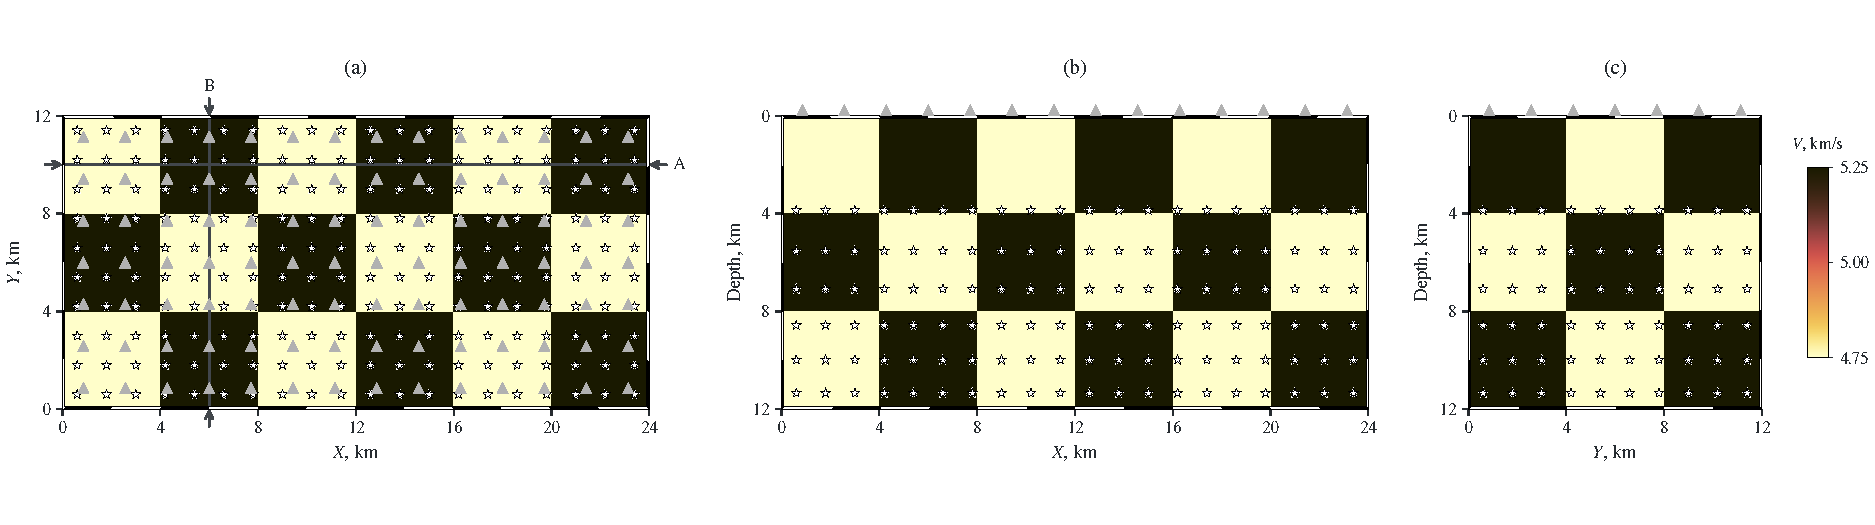
\includegraphics[width=\textwidth]{figures/used/checkerboard_nx6_geometry.pdf}
\begin{singlespace}
\caption{Checkerboard geometry for $n_x=6$: (a) plan view with section traces A and B; (b,c) vertical sections A and B, respectively. Grey triangles and white stars show projected stations and events; overlapping projections are drawn once. Depth is positive downward.}
\label{fig:checkerboard_geometry_current}
\end{singlespace}
\end{figure}

Whole-volume velocity errors, evaluated on a common 31.25-m grid, are 151--175~m/s RMSE and 2.3--2.8\% MAPE for EMTomo, and 199--221~m/s and 3.0--3.7\% for tomoDD (Table~\ref{tab:checkerboard_metrics}). Hypocenter P90 is 373--506~m and 588--609~m, respectively. Both methods recover the main structure, but their different parameterizations and inversion settings prevent attributing the error difference to one algorithmic feature. Figures~\ref{fig:checkerboard_comparison_current} and~\ref{fig:checkerboard_locations} show the recovered models and example locations.

\begin{table}[!htb]
\centering
\begin{singlespace}
\small
\setlength{\tabcolsep}{3.5pt}
% Velocity: figures/checkerboard_velocity_metrics.json (RMSE) and figures/table_supplementary_metrics.json (MAPE).
\caption{Checkerboard with full coverage: whole-volume velocity errors on a common 31.25-m grid and hypocenter P90 over all 1200 events. Initial errors are 250~m/s RMSE and 5.0\% MAPE. Oracle is the trilinear oracle for the tomoDD parameterization; the constant-cell oracle error of EMTomo is zero because the boundaries align. EMTomo locations precede the twelfth velocity update; tomoDD locations follow three joint iterations.}
\label{tab:checkerboard_metrics}
\smallskip
\begin{tabular}{rrrrrrrrr}
\toprule
& \multicolumn{3}{c}{Velocity RMSE (m/s)} & \multicolumn{3}{c}{Velocity MAPE (\%)} & \multicolumn{2}{c}{P90 (m)} \\
\cmidrule(lr){2-4}\cmidrule(lr){5-7}\cmidrule(lr){8-9}
$n_x$ & EMTomo & tomoDD & Oracle & EMTomo & tomoDD & Oracle & EMTomo & tomoDD \\
\midrule
4 & 175.3 & 199.2 & 76.2 & 2.81 & 2.99 & 0.97 & 505.9 & 599.2 \\
6 & 155.7 & 215.1 & 98.8 & 2.40 & 3.47 & 1.31 & 373.4 & 588.1 \\
8 & 150.8 & 221.2 & 117.4 & 2.34 & 3.69 & 1.81 & 402.5 & 609.1 \\
\bottomrule
\end{tabular}
\end{singlespace}
\end{table}

\begin{figure}[!htb]
\centering
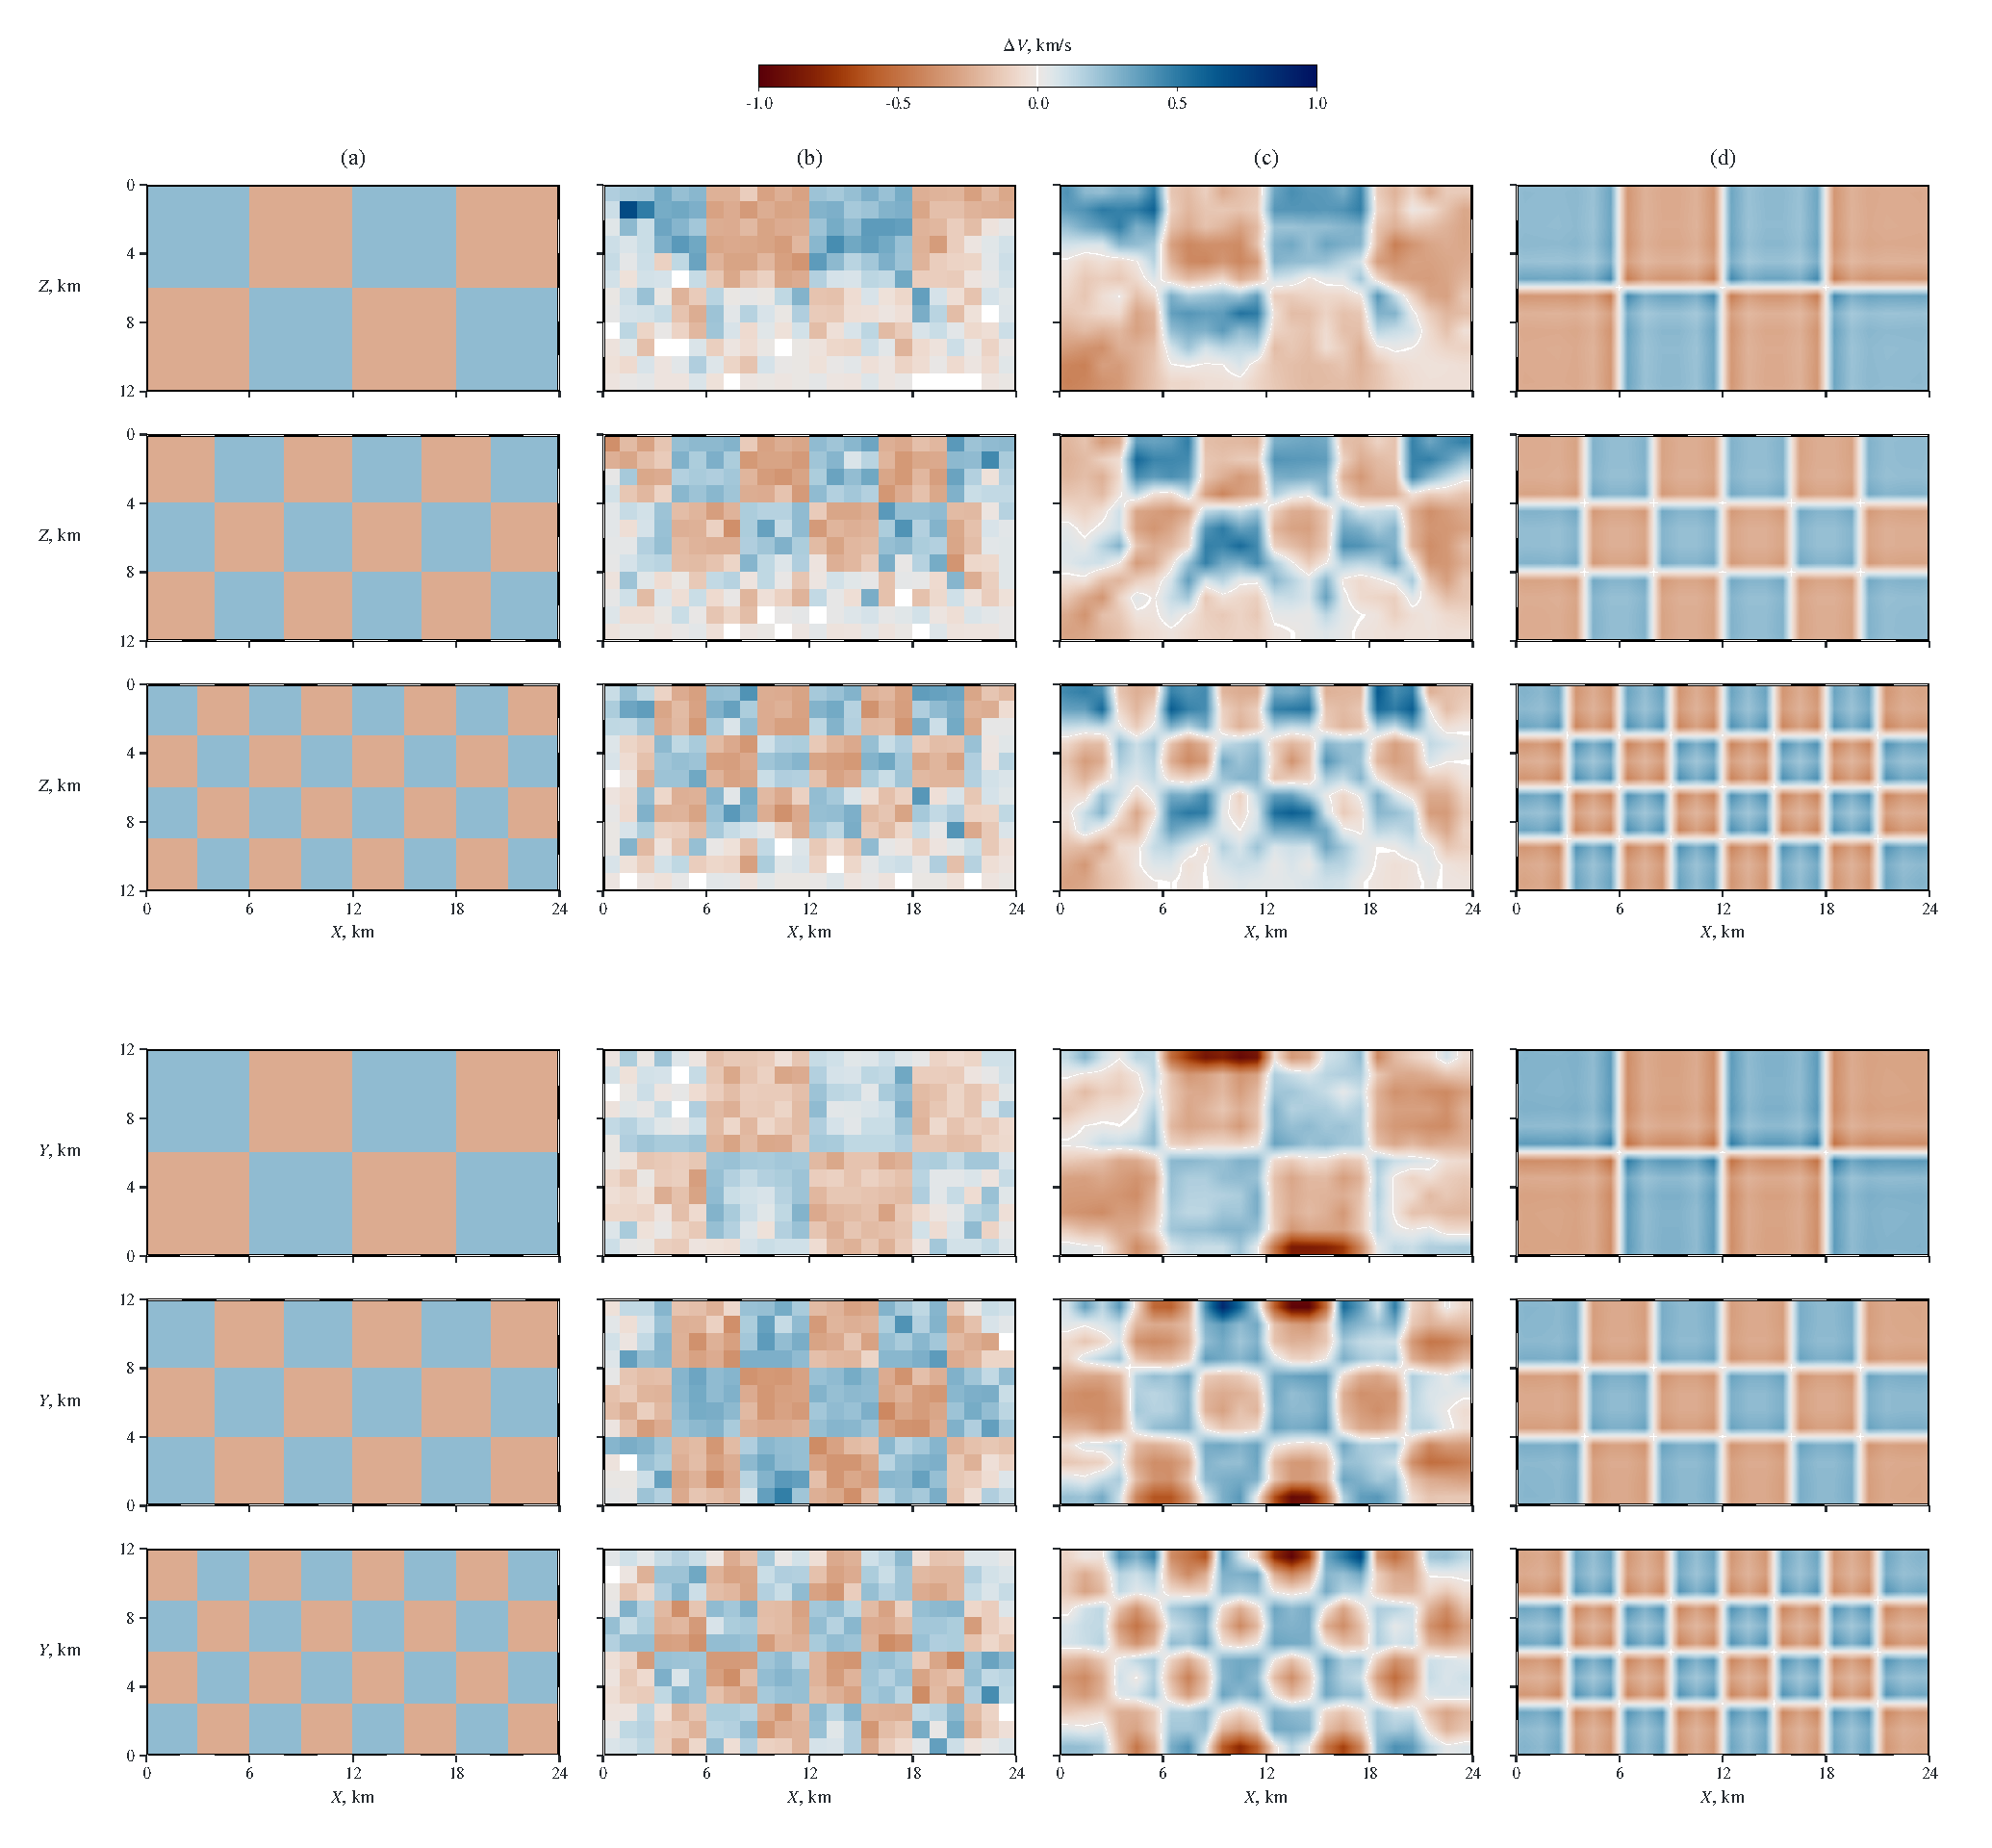
\includegraphics[width=\textwidth,height=0.62\textheight,keepaspectratio]{figures/used/checkerboard_nx4_nx6_nx8_comparison.pdf}
\begin{singlespace}
\caption{Checkerboard models by column: (a) truth; (b) EMTomo after 12 updates; (c) tomoDD after three iterations; (d) truth-only trilinear oracle. Upper three rows: vertical sections at $Y=10$~km; lower three: horizontal sections at $Z=5$~km. In each group, $n_x=4,6,8$ from top to bottom. Colors show $\Delta V=V-5$~km/s; white denotes zero perturbation.}
\label{fig:checkerboard_comparison_current}
\end{singlespace}
\end{figure}
\FloatBarrier

\begin{figure}[!htb]
\centering
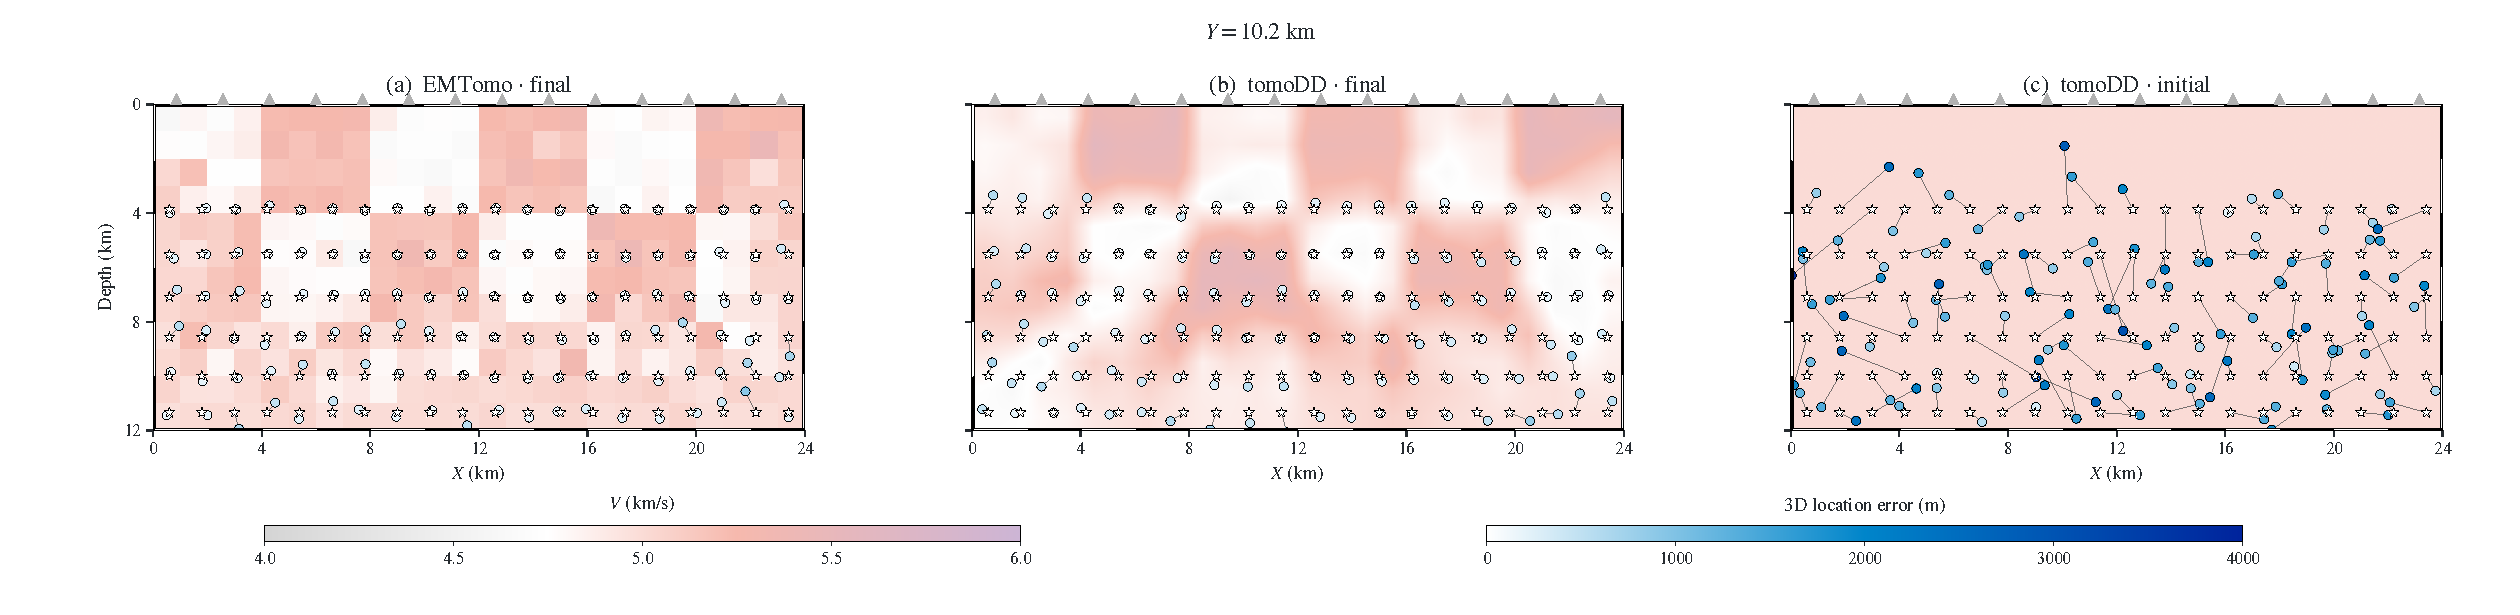
\includegraphics[width=\textwidth]{figures/used/checkerboard_nx6_locations_y10p2km.pdf}
\begin{singlespace}
\caption{Locations of 120 events at true $Y=10.2$~km for $n_x=6$: (a) EMTomo, (b) tomoDD, (c) initial tomoDD locations. Stars and circles show truth and estimates projected onto the $X$--depth plane; colors give full 3D errors. Backgrounds show the corresponding velocity models. EMTomo locations precede the last velocity update.}
\label{fig:checkerboard_locations}
\end{singlespace}
\end{figure}
\FloatBarrier

\subsection{Checkerboard with One-sided Station Coverage}
\label{subsec:onesided_results}

This test compares hard and soft assignment when stations lie on one side of the source region and event locations are poorly constrained.

The $n_x=6$ checkerboard contains 1200 events and 18 surface stations at $X=1.4$--$4.5$~km; 900 events lie farther away, at $X=10$--$21$~km. Shared picks have 1\% relative and 0.05~s absolute Gaussian noise. Runs start from 5~km/s and use 1-km cells, $q=8$, 12 updates, $\lambda=1$, $\gamma=2$, a 2\% step limit, and 0.02~s model uncertainty. Candidate seeds are separated by 875~m. Hard uses the best of 50 or 100 tested candidates; soft retains the counts listed in Table~\ref{tab:onesided_comparison}.

The reported models are taken after three updates for every run. Soft has lower velocity RMSE and MAPE in all four comparisons, but lower location P90 only when retaining 10 or 25 candidates. With at least 25 candidates, its velocity RMSE also falls below the initial 250~m/s. Residual RMS is almost the same in both modes, 0.0498--0.0506~s for soft and 0.0499~s for hard. The hard-50 control is reused, so these comparisons are not independent repeats. Using the weighted mean of the soft candidate coordinates instead of the largest-weight candidate gives a clearer location improvement: P90 falls to 5.23--5.61~km, compared with 6.16~km for hard assignment (Table~\ref{tab:onesided_comparison}). All four soft variants then outperform hard in P90; the velocity results are unchanged.

\begin{table}[!htb]
\centering
\begin{singlespace}
\small
\setlength{\tabcolsep}{3.5pt}
% L-curve metrics and checkpoints: figures/hard_soft_lcurve_comparison_metrics.json, onesided; MAPE, residuals and weighted-mean P90: figures/table_supplementary_metrics.json.
\caption{One-sided coverage after three updates for every run. Tested and used count searched candidates and locations contributing to the update. P90 covers all 1200 events relocated in the selected model. Residual RMS and P90 refer to the location step in the reported model; the weighted-mean P90 is given for soft only. Max. wt.: largest-weight candidate; Mean: weighted mean of the retained candidates; Mode: hard or soft assignment.}
\label{tab:onesided_comparison}
\smallskip
\begin{tabular}{lllrrrrr}
\toprule
& & & \multicolumn{2}{c}{Velocity} & Residual & \multicolumn{2}{c}{P90 (m)} \\
\cmidrule(lr){4-5}\cmidrule(lr){7-8}
Mode & Tested & Used & RMSE (m/s) & MAPE (\%) & RMS (s) & Max.\ wt. & Mean \\
\midrule
Hard & 50 & 1 & 256.4 & 4.89 & 0.0499 & 6160.8 & --- \\
Soft & 50 & 10 & 251.5 & 4.85 & 0.0498 & 6019.1 & 5612.1 \\
Soft & 50 & 25 & 248.4 & 4.84 & 0.0501 & 6112.1 & 5391.7 \\
Soft & 50 & 50 & 246.8 & 4.83 & 0.0504 & 6222.3 & 5248.0 \\
\addlinespace
Hard & 100 & 1 & 256.4 & 4.89 & 0.0499 & 6160.8 & --- \\
Soft & 100 & 100 & 245.8 & 4.82 & 0.0506 & 6390.3 & 5231.3 \\
\bottomrule
\end{tabular}
\end{singlespace}
\end{table}

\begin{figure}[!htbp]
\centering
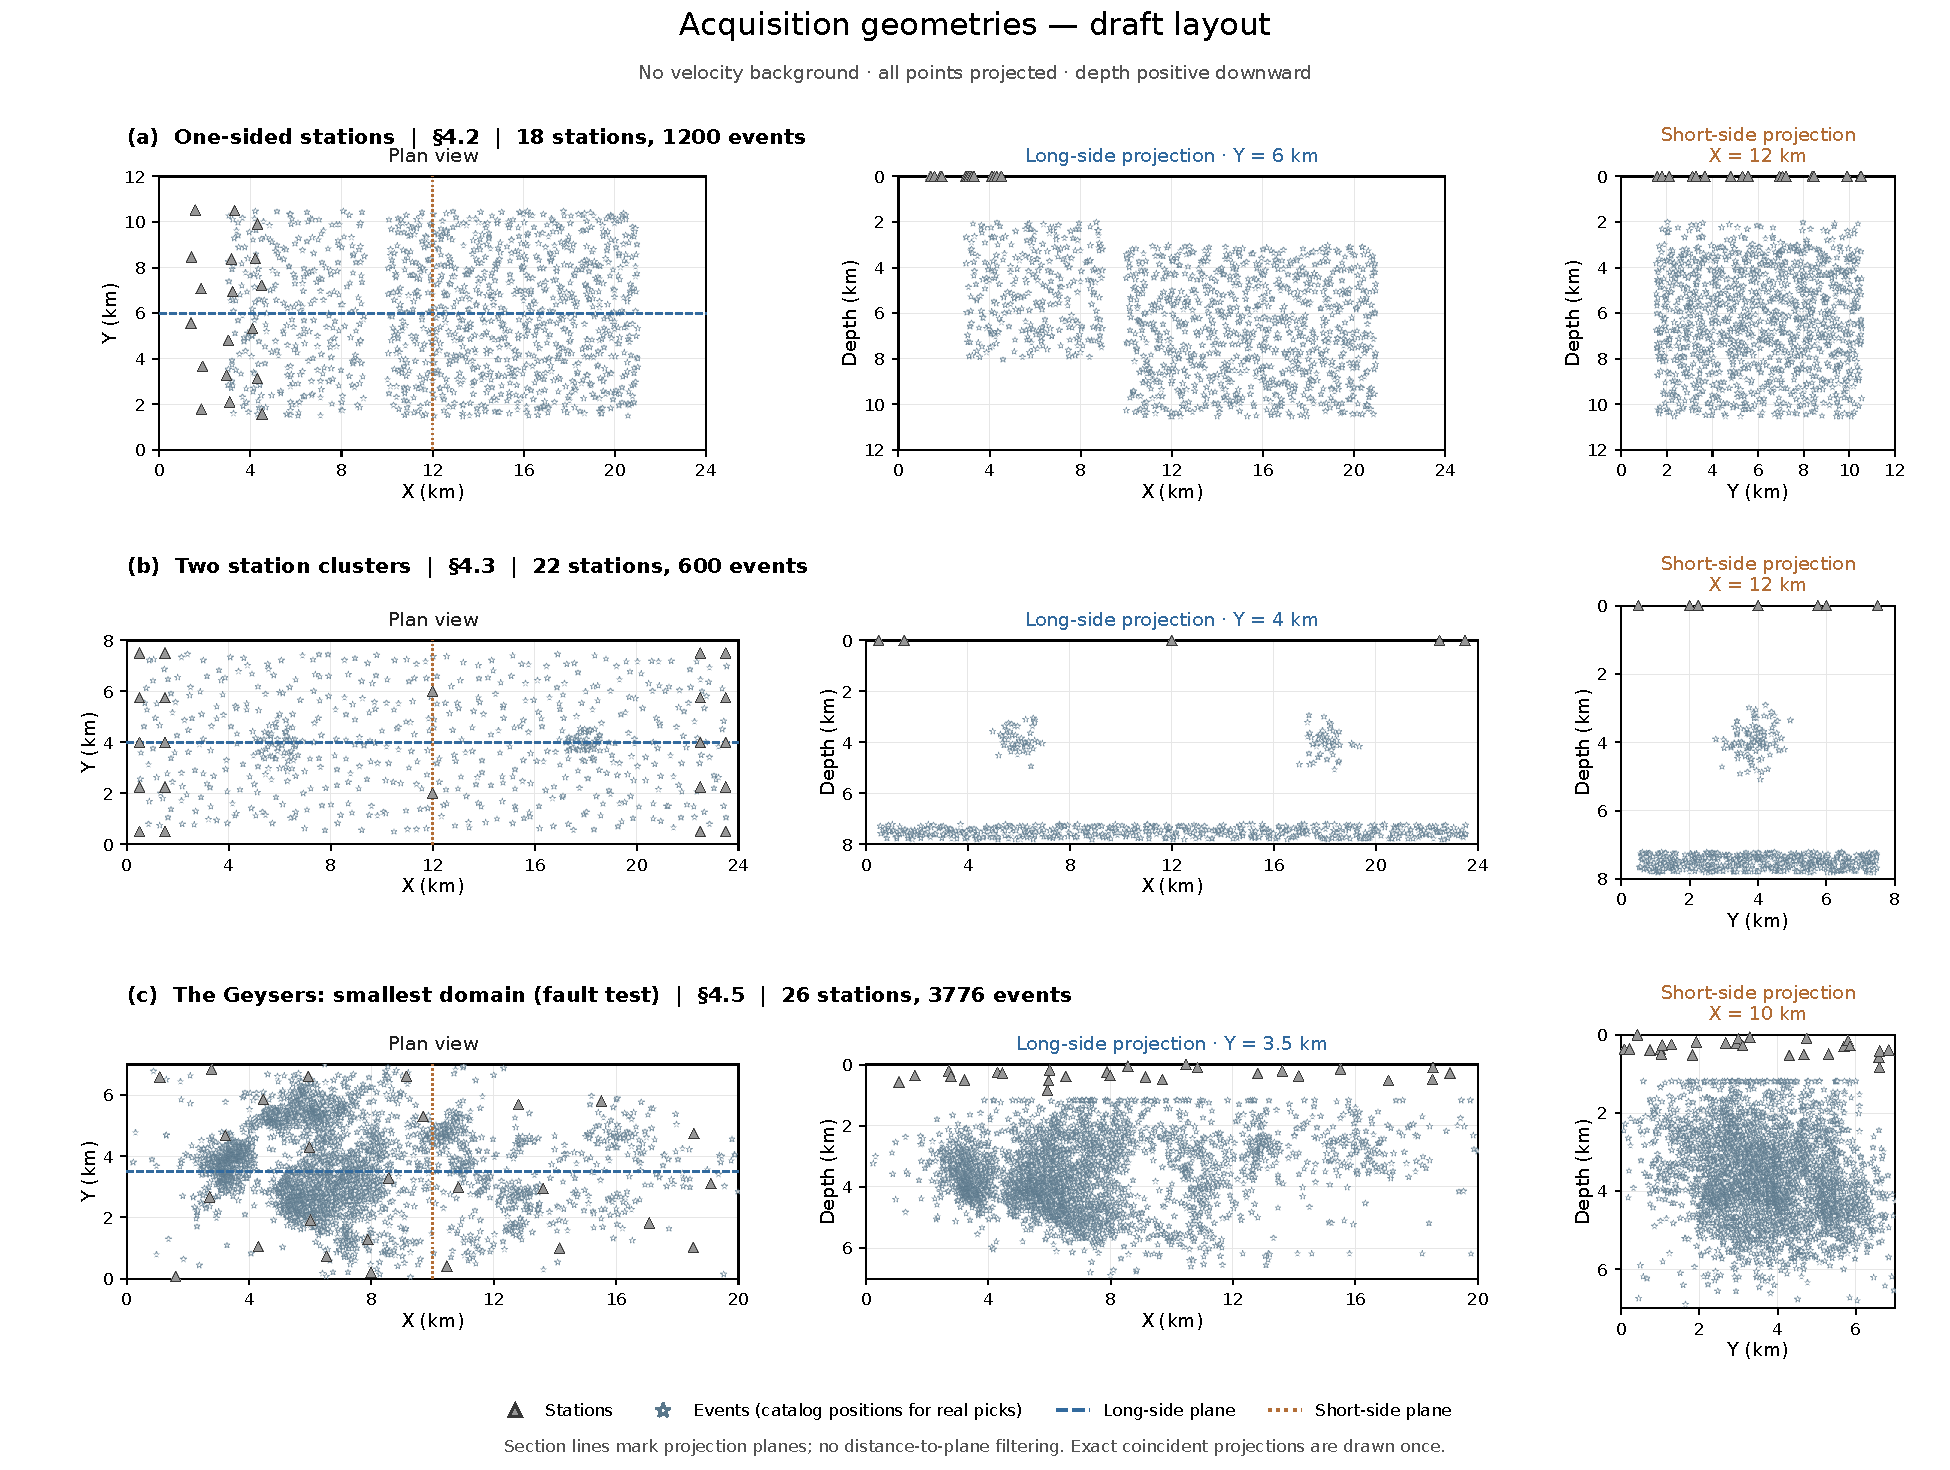
\includegraphics[width=\textwidth]{figures/used/all_geometries.pdf}
\begin{singlespace}
\caption{Acquisition geometries (draft). Rows show (a) one-sided stations, (b) two station clusters, and (c) The Geysers geometry for the fault test, with the smallest real-derived model domain. Columns show the plan view and projections onto vertical planes along the long and short sides of each domain. Triangles denote stations and stars denote events. Lines in the plan views mark the projection planes; all points are projected, without distance filtering. Depth is positive downward. The other real-derived tests use different domain bounds and event selections.}
\label{fig:additional_geometries}
\end{singlespace}
\end{figure}
\FloatBarrier

\subsection{Checkerboard with Two Station Clusters}
\label{subsec:two_clusters_results}

This test places stations on both sides of a mainly deep event population in a $24\times8\times8$~km checkerboard with 4-km cubes at 4.75 and 5.25~km/s. Ten stations lie near each end along $X$, with two in the middle. Of 600 events, 500 lie at depths of 7.2--7.8~km; two clusters of 50 lie near $(6,4,4)$ and $(18,4,4)$~km. Noise, starting model, grids, and inversion settings follow Section~\ref{subsec:onesided_results}, including reuse of the hard-50 control.

All runs select three updates. Soft slightly reduces velocity RMSE and MAPE but increases location P90 (Table~\ref{tab:two_clusters_comparison}); residual RMS differs by only 0.1~ms. The weighted mean lowers the soft P90 to 1413--1416~m, still above the 1340~m of hard assignment. Both modes remain above the initial 250~m/s, and retaining more candidates gives little further benefit.

\begin{table}[!htb]
\centering
\begin{singlespace}
\small
\setlength{\tabcolsep}{3.5pt}
% L-curve metrics and checkpoints: figures/hard_soft_lcurve_comparison_metrics.json, two_clusters; supplementary metrics: figures/table_supplementary_metrics.json.
\caption{Two station clusters after three updates for every run. Metrics and candidate counts follow Table~\ref{tab:onesided_comparison}; P90 covers all 600 events.}
\label{tab:two_clusters_comparison}
\smallskip
\begin{tabular}{lllrrrrr}
\toprule
& & & \multicolumn{2}{c}{Velocity} & Residual & \multicolumn{2}{c}{P90 (m)} \\
\cmidrule(lr){4-5}\cmidrule(lr){7-8}
Mode & Tested & Used & RMSE (m/s) & MAPE (\%) & RMS (s) & Max.\ wt. & Mean \\
\midrule
Hard & 50 & 1 & 253.7 & 4.76 & 0.0523 & 1340.4 & --- \\
Soft & 50 & 10 & 251.3 & 4.74 & 0.0524 & 1467.3 & 1412.6 \\
Soft & 50 & 25 & 251.3 & 4.74 & 0.0524 & 1468.4 & 1416.3 \\
Soft & 50 & 50 & 251.3 & 4.74 & 0.0524 & 1469.1 & 1414.7 \\
\addlinespace
Hard & 100 & 1 & 253.7 & 4.76 & 0.0523 & 1340.4 & --- \\
Soft & 100 & 100 & 251.3 & 4.74 & 0.0524 & 1469.3 & 1415.2 \\
\bottomrule
\end{tabular}
\end{singlespace}
\end{table}
\FloatBarrier

\begin{figure}[!htbp]
\centering
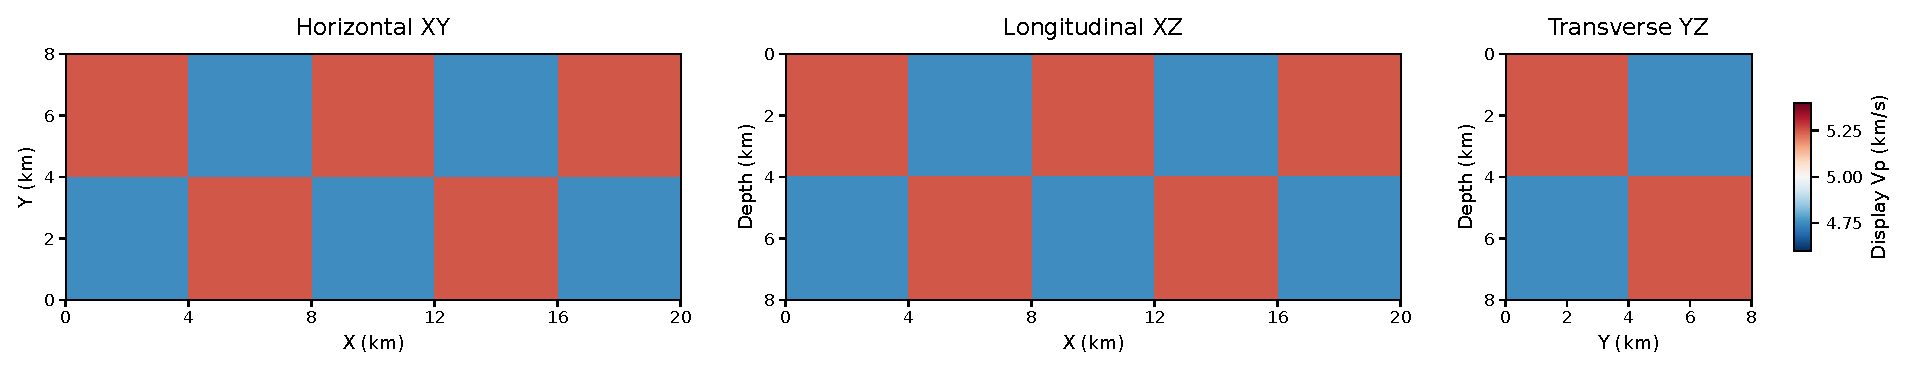
\includegraphics[width=\textwidth]{figures/used/checkerboards_4_2-4_4_true_final.pdf}
\begin{singlespace}
\caption{Common displayed checkerboard patterns for Sections~\ref{subsec:onesided_results}--\ref{subsec:checkerboard_noise_results}. Left to right: horizontal $XY$ at $Z=1.5$~km, longitudinal $XZ$ at $Y=4.5$~km, and transverse $YZ$ at $X=4.5$~km. The one-sided and two-cluster domains are cropped at the right edge to $X=0$--20~km; the one-sided domain is also cropped to $Y,Z=0$--8~km. Axes use native model coordinates. For the realistic-geometry checkerboard only, the displayed anomaly sign is reversed about 5~km/s, $V_P^{\mathrm{disp}}=10~\mathrm{km/s}-V_P$, yielding identical displayed patterns. This is a plotting convention, not a change to the physical truth or inversion.}
\label{fig:checkerboards_common_true}
\end{singlespace}
\end{figure}

\begin{figure}[!htbp]
\centering
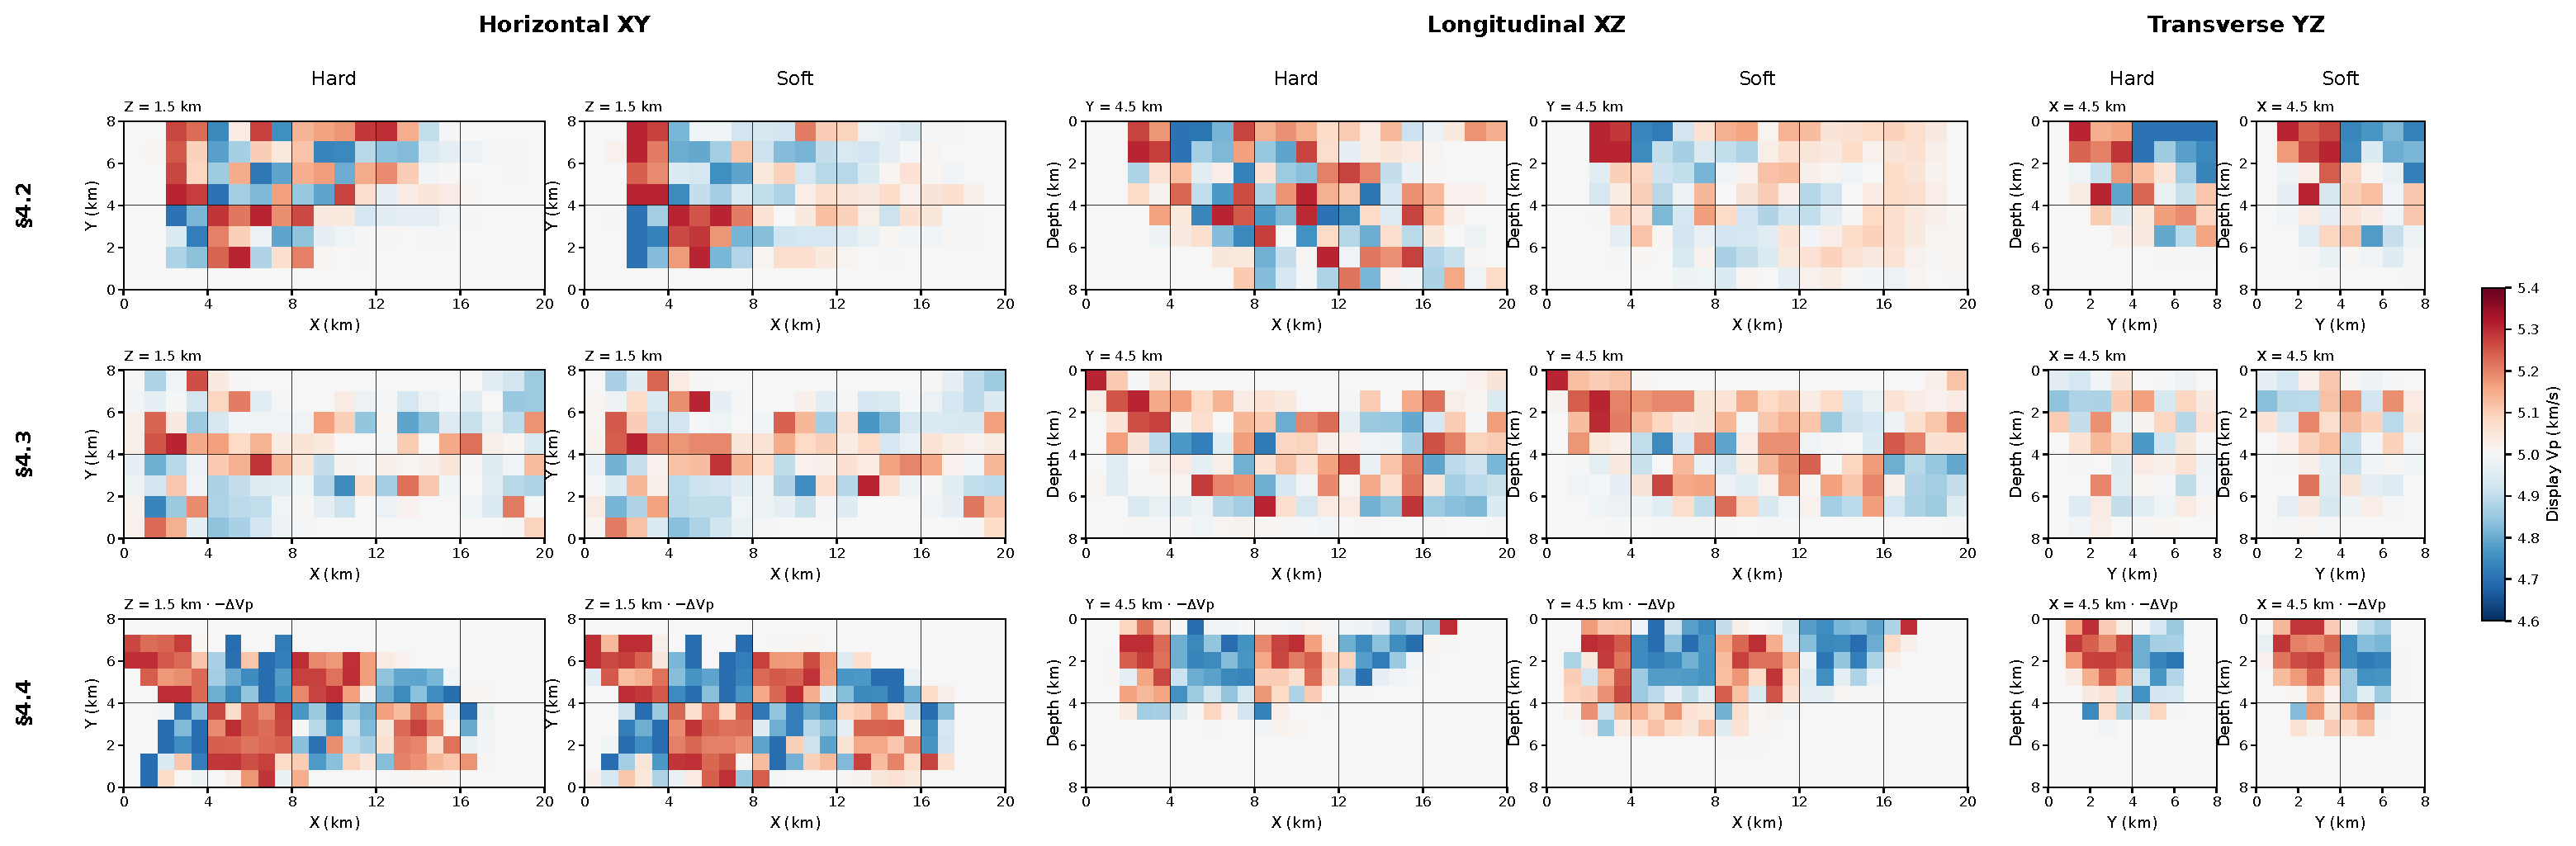
\includegraphics[width=\textwidth]{figures/used/checkerboards_4_2-4_4_results_final.pdf}
\begin{singlespace}
\caption{Hard and soft checkerboard reconstructions after three updates. Rows correspond to one-sided stations, two station clusters, and realistic geometry (Sections~\ref{subsec:onesided_results}--\ref{subsec:checkerboard_noise_results}); paired columns show hard and soft for $XY$, $XZ$, and $YZ$, respectively. Crops, section coordinates, and the shared color scale follow Figure~\ref{fig:checkerboards_common_true}. Thin black lines mark true checkerboard interfaces. The bottom row uses the same anomaly-sign reversal as its displayed truth, explicitly marked $-\Delta V_P$; all other rows retain their original signs. Native cell values are shown without smoothing. Quantitative errors in the tables refer to the original, untransformed full-domain models, not these cropped display fields.}
\label{fig:checkerboards_hard_soft_final}
\end{singlespace}
\end{figure}
\FloatBarrier

\subsection{Checkerboard with Realistic Geometry}
\label{subsec:checkerboard_noise_results}

This test uses event coordinates from the Berkeley Geysers (BG) catalog in the NCEDC Enhanced Geothermal Systems archive, and station coordinates and elevations from the NCEDC FDSN Station service \parencite{ncedc2014}. A $20\times8\times8$~km checkerboard with 4-km cubes at 4.75 and 5.25~km/s contains 26 stations and 3465 events. PyKonal generates all 90,090 arrivals on a 100-m grid. Catalog coordinates define synthetic truth; neither real picks nor their missing-data pattern are used.

The inversion uses 800-m cells, $q=8$, and 700-m seed separation; other settings follow Section~\ref{subsec:onesided_results}. With 50 tested candidates, we scale both noise components by 0.5--2 relative to 1\% and 0.05~s, keeping the likelihood noise fixed. The same noise realization is scaled in all cases. A second test varies the candidate count from 30 to 200 at nominal noise. Soft retains all tested candidates.

All runs select three updates. Soft has lower velocity RMSE and MAPE but higher location P90 at every noise level (Table~\ref{tab:real_geometry_noise}). This also holds for the weighted-mean P90, while residual RMS agrees between the modes to within 0.1~ms. All selected velocity models improve on the initial 250~m/s. More candidates slightly reduce soft velocity RMSE but increase P90; hard changes little (Table~\ref{tab:real_geometry_candidates}). The nominal-noise, 50-candidate pair is shared by both tables.

\begin{table}[!htb]
\centering
\begin{singlespace}
\small
\setlength{\tabcolsep}{3.5pt}
% L-curve metrics and checkpoints: figures/hard_soft_lcurve_comparison_metrics.json, real_geometry_noise; supplementary metrics: figures/table_supplementary_metrics.json.
\caption{Realistic geometry: noise sweep with 50 candidates, evaluated after the selected three updates. Noise factors scale both 1\% relative and 0.05~s absolute standard deviations. P90 covers all 3465 events. Metrics follow Table~\ref{tab:onesided_comparison}.}
\label{tab:real_geometry_noise}
\smallskip
\begin{tabular}{llrrrrr}
\toprule
& & \multicolumn{2}{c}{Velocity} & Residual & \multicolumn{2}{c}{P90 (m)} \\
\cmidrule(lr){3-4}\cmidrule(lr){6-7}
Noise & Mode & RMSE (m/s) & MAPE (\%) & RMS (s) & Max.\ wt. & Mean \\
\midrule
0.5 & Hard & 230.8 & 4.40 & 0.0246 & 378.6 & --- \\
 & Soft & 228.2 & 4.29 & 0.0245 & 448.5 & 472.2 \\
\addlinespace
0.75 & Hard & 231.1 & 4.40 & 0.0364 & 514.6 & --- \\
 & Soft & 228.7 & 4.30 & 0.0363 & 593.8 & 609.0 \\
\addlinespace
1 & Hard & 232.0 & 4.41 & 0.0483 & 665.3 & --- \\
 & Soft & 229.6 & 4.31 & 0.0483 & 755.9 & 765.6 \\
\addlinespace
1.5 & Hard & 235.3 & 4.45 & 0.0721 & 1005.6 & --- \\
 & Soft & 232.7 & 4.34 & 0.0721 & 1098.8 & 1085.9 \\
\addlinespace
2 & Hard & 239.3 & 4.49 & 0.0960 & 1364.5 & --- \\
 & Soft & 237.8 & 4.41 & 0.0960 & 1496.9 & 1465.7 \\
\bottomrule
\end{tabular}
\end{singlespace}
\end{table}

\begin{table}[!htb]
\centering
\begin{singlespace}
\small
\setlength{\tabcolsep}{3.5pt}
% L-curve metrics and checkpoints: figures/hard_soft_lcurve_comparison_metrics.json, real_geometry_candidates; supplementary metrics: figures/table_supplementary_metrics.json.
\caption{Candidate-count sweep at nominal noise, using the same selection and metrics as Table~\ref{tab:real_geometry_noise}. Hard uses one candidate; soft uses all tested candidates. The 50-candidate pair is reused.}
\label{tab:real_geometry_candidates}
\smallskip
\begin{tabular}{llrrrrr}
\toprule
& & \multicolumn{2}{c}{Velocity} & Residual & \multicolumn{2}{c}{P90 (m)} \\
\cmidrule(lr){3-4}\cmidrule(lr){6-7}
Tested & Mode & RMSE (m/s) & MAPE (\%) & RMS (s) & Max.\ wt. & Mean \\
\midrule
30 & Hard & 232.0 & 4.41 & 0.0483 & 665.3 & --- \\
 & Soft & 229.8 & 4.32 & 0.0483 & 752.5 & 762.8 \\
\addlinespace
50 & Hard & 232.0 & 4.41 & 0.0483 & 665.3 & --- \\
 & Soft & 229.6 & 4.31 & 0.0483 & 755.9 & 765.6 \\
\addlinespace
100 & Hard & 232.0 & 4.41 & 0.0483 & 665.3 & --- \\
 & Soft & 229.4 & 4.30 & 0.0483 & 757.5 & 767.4 \\
\addlinespace
150 & Hard & 232.0 & 4.41 & 0.0483 & 665.3 & --- \\
 & Soft & 229.4 & 4.30 & 0.0483 & 759.0 & 768.0 \\
\addlinespace
200 & Hard & 232.0 & 4.41 & 0.0483 & 665.3 & --- \\
 & Soft & 229.4 & 4.30 & 0.0482 & 759.2 & 767.8 \\
\bottomrule
\end{tabular}
\end{singlespace}
\end{table}
\FloatBarrier

\subsection{Vertical Fault with Realistic Geometry}
\label{subsec:fault_results}

We test a sharp lateral discontinuity in a $20\times7\times7$~km model with 26 stations and 3776 events, using The Geysers geometry from NCEDC \parencite{ncedc2014}. A vertical fault at $X=6.5$~km separates two three-layer blocks with different interface depths and velocities of 3.6--5.5~km/s. The truth uses 125-m voxels; PyKonal generates all 98,176 arrivals at 62.5-m spacing. All runs share Gaussian pick noise of 2\% relative and 0.02~s absolute standard deviation.

The layered start has velocities of 3.85, 4.55, and 5.30~km/s and interfaces at 0.85 and 2.3~km. Runs use 1-km cells, $q=8$, 128 tested candidates, unit temperature, $\lambda=1$, $\gamma=0$, a 2\% step limit, and 12 updates. The likelihood uses the nominal pick noise plus 0.02~s model uncertainty. We vary retained count and seed separation while keeping these settings fixed.

At 250-m separation, soft has higher velocity RMSE and MAPE but lower location P90 (Table~\ref{tab:fault_retention}). This location advantage holds only for the largest-weight candidate: the weighted-mean P90 of 469--487~m is not below the 467.8~m of hard assignment. Residual RMS is 0.0365~s for soft and 0.0364~s for hard. More retained candidates do not improve velocity recovery. All final models improve on the initial 277.1~m/s.

\begin{table}[!htb]
\centering
\begin{singlespace}
\small
\setlength{\tabcolsep}{3.5pt}
% Final-model metrics: figures/final_comparison_metrics.json, fault_retention; supplementary metrics: figures/table_supplementary_metrics.json.
\caption{Fault model: retained-count sweep with 128 tested candidates and 250-m separation. Final models after 12 updates in both modes. P90 covers all 3776 events, located in the E-step preceding the twelfth update; residuals come from the same step. The hard control is reused. Metrics follow Table~\ref{tab:onesided_comparison}.}
\label{tab:fault_retention}
\smallskip
\begin{tabular}{llrrrrr}
\toprule
& & \multicolumn{2}{c}{Velocity} & Residual & \multicolumn{2}{c}{P90 (m)} \\
\cmidrule(lr){3-4}\cmidrule(lr){6-7}
Mode & Used & RMSE (m/s) & MAPE (\%) & RMS (s) & Max.\ wt. & Mean \\
\midrule
Hard & 1 & 260.4 & 4.71 & 0.0364 & 467.8 & --- \\
Soft & 40 & 265.4 & 4.81 & 0.0365 & 458.9 & 469.3 \\
Soft & 50 & 266.0 & 4.81 & 0.0365 & 459.9 & 476.2 \\
Soft & 75 & 266.4 & 4.82 & 0.0365 & 465.1 & 485.1 \\
Soft & 100 & 266.5 & 4.82 & 0.0365 & 465.6 & 486.3 \\
Soft & 128 & 266.6 & 4.82 & 0.0365 & 463.8 & 487.1 \\
\bottomrule
\end{tabular}
\end{singlespace}
\end{table}

Wider seed separation improves the soft velocity result (Table~\ref{tab:fault_separation}). At 875~m, soft is slightly better in velocity RMSE, MAPE, and P90. At both wider separations, the weighted mean lowers the soft P90 further, to 424~m at 500~m and 441~m at 875~m. Retaining 128 rather than 50 candidates has negligible effect. The result supports testing candidate spacing, but does not establish a universal optimum.

\begin{table}[!htb]
\centering
\begin{singlespace}
\small
\setlength{\tabcolsep}{3.5pt}
% Final-model metrics: figures/final_comparison_metrics.json, fault_separation; supplementary metrics: figures/table_supplementary_metrics.json.
\caption{Fault model: seed-separation sweep with 128 tested candidates. Retained is the soft count; each soft run has its own matched hard control, which uses one candidate. Final models after 12 updates in both modes; timing and metrics follow Table~\ref{tab:fault_retention}.}
\label{tab:fault_separation}
\smallskip
\begin{tabular}{lllrrrrr}
\toprule
& & & \multicolumn{2}{c}{Velocity} & Residual & \multicolumn{2}{c}{P90 (m)} \\
\cmidrule(lr){4-5}\cmidrule(lr){7-8}
Sep. (m) & Retained & Mode & RMSE (m/s) & MAPE (\%) & RMS (s) & Max.\ wt. & Mean \\
\midrule
500 & 50 & Hard & 260.3 & 4.71 & 0.0364 & 464.1 & --- \\
 &  & Soft & 263.0 & 4.76 & 0.0365 & 434.0 & 423.5 \\
\addlinespace
 & 128 & Hard & 260.3 & 4.71 & 0.0364 & 464.1 & --- \\
 &  & Soft & 263.0 & 4.76 & 0.0365 & 434.0 & 423.5 \\
\addlinespace
875 & 50 & Hard & 260.3 & 4.71 & 0.0364 & 463.8 & --- \\
 &  & Soft & 259.3 & 4.70 & 0.0364 & 446.6 & 441.3 \\
\addlinespace
 & 128 & Hard & 260.3 & 4.71 & 0.0364 & 463.8 & --- \\
 &  & Soft & 259.3 & 4.70 & 0.0364 & 446.6 & 441.3 \\
\bottomrule
\end{tabular}
\end{singlespace}
\end{table}
\begin{figure}[!htbp]
\centering
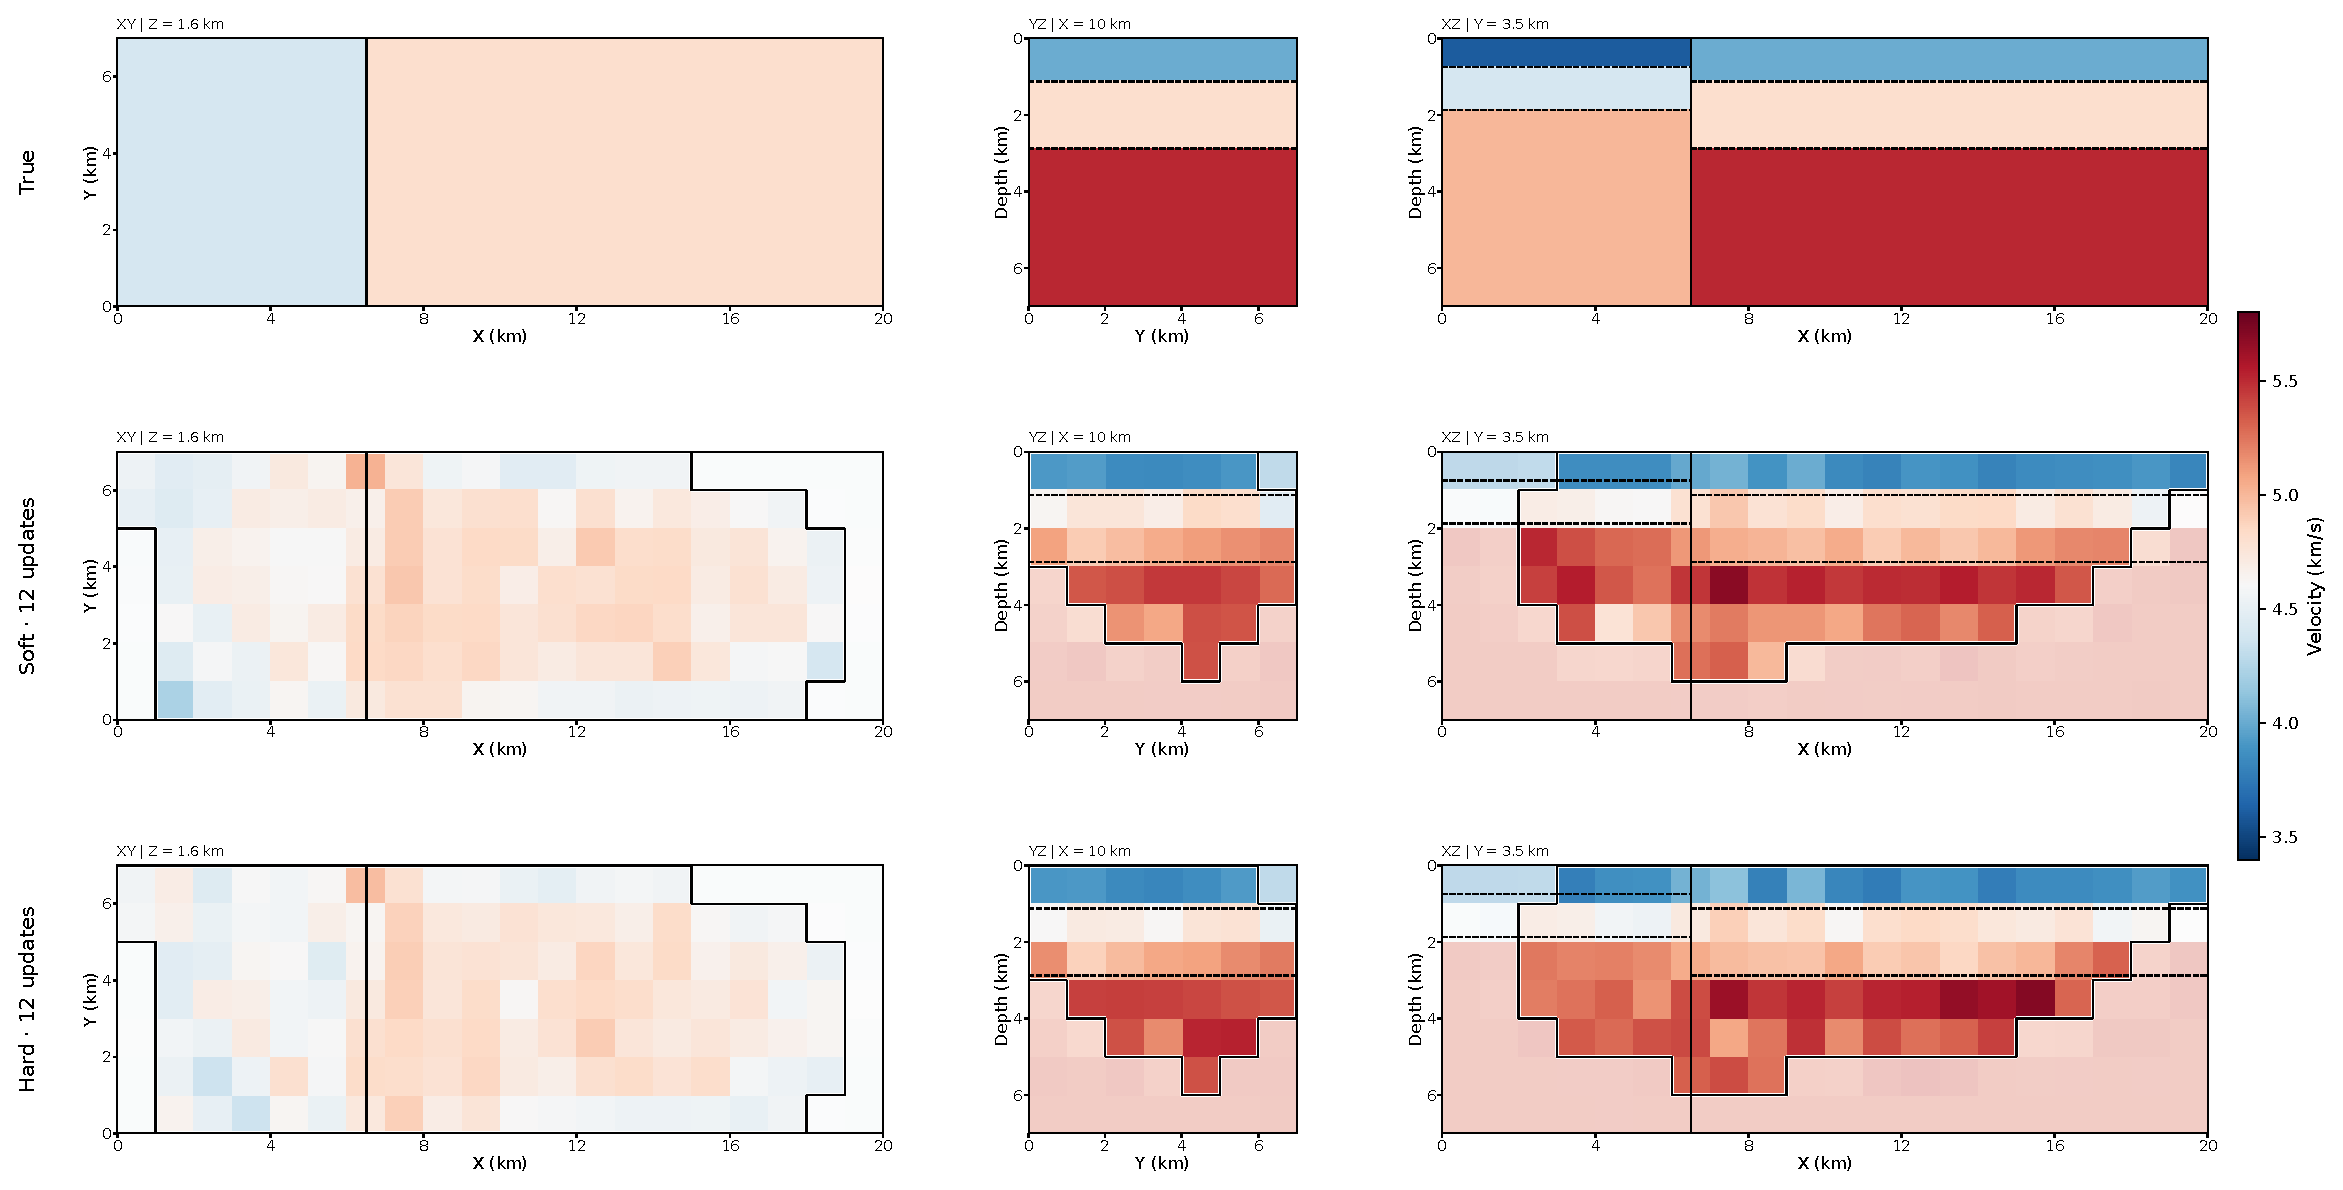
\includegraphics[width=\textwidth,height=0.63\textheight,keepaspectratio]{figures/used/section_4_5_final.pdf}
\begin{singlespace}
\caption{Vertical-fault model: truth, final soft reconstruction, and final hard reconstruction (top to bottom). Columns show $XY$ at $Z=1.6$~km, $YZ$ at $X=10$~km, and $XZ$ at $Y=3.5$~km. Both reconstructions use 12 updates; soft retains 50 of 128 tested candidates at 250-m seed separation. These are the models of the hard row and the 50-candidate soft row in Table~\ref{tab:fault_retention}. Solid black lines mark the source fault at $X=6.5$~km; dashed lines mark source layer interfaces. The identical hard/soft display envelope is the filled convex hull of their common diagonal-sensitivity selection $H_{jj}/\alpha\geq1$, expanded by one 1-km cell, where $\alpha=\lambda\,\mathrm{mean}(H_{jj})$. Outside it, velocities are faded. This envelope is not a spatial-resolution test; added cells may fail the threshold, and diagnostics precede the final update. Native cell values are not smoothed.}
\label{fig:fault_sections_final}
\end{singlespace}
\end{figure}
\FloatBarrier

\subsection{Heterogeneous Model with Realistic Geometry}
\label{subsec:heterogeneous_results}

This test replaces the checkerboard in Section~\ref{subsec:checkerboard_noise_results} with a heterogeneous upper-crust model in the same $20\times8\times8$~km domain. It combines a depth gradient, an undulating basin, a dipping low-velocity fault zone, a high-velocity intrusion, and a low-velocity lens. The NCEDC-derived geometry of 26 stations and 3465 events \parencite{ncedc2014} and the nominal noise levels are unchanged. New synthetic arrivals are generated for all event--station pairs. Truth and forward computation use a 100-m grid.

Runs use 800-m inversion cells, $q=8$, 50 tested candidates, 700-m seed separation, $\lambda=1$, $\gamma=0$, unit temperature, and a 2\% step limit. Hard uses one candidate and soft uses all 50. We compare a homogeneous 5~km/s start with a 1-D profile obtained by horizontally averaging and depth-smoothing the truth; the latter is a favorable, truth-informed start. A fixed 10\% of picks is held out. Control-RMSE stopping ends the 1-D runs after nine updates; homogeneous runs reach the limit of 20. We report the final models at these stopping points (Table~\ref{tab:heterogeneous_comparison}).

The starting model has a much larger effect than hard versus soft assignment (Table~\ref{tab:heterogeneous_comparison}). Both modes slightly reduce velocity RMSE from their respective starts. Soft is 2.1~m/s better than hard from the 1-D start but 6.2~m/s worse from the homogeneous start, so it gives no consistent velocity advantage; MAPE follows the same pattern. Its location P90 is higher in both cases, especially from the homogeneous start, and the weighted mean does not change this. Residual RMS is similar, at 0.0494 versus 0.0495~s and 0.0548 versus 0.0556~s for hard versus soft. Thus, source-location averaging alone does not resolve a poor initial velocity model in this test.

\begin{table}[!htb]
\centering
\begin{singlespace}
\small
\setlength{\tabcolsep}{3.5pt}
% Final-model metrics: figures/final_comparison_metrics.json, heterogeneous; cap20 pairs only; supplementary metrics: figures/table_supplementary_metrics.json.
\caption{Heterogeneous model: final models after nine updates for the 1-D start (control-RMSE stopping) and 20 for the homogeneous start (update limit). Initial whole-volume RMSE is 504.0 and 1074.9~m/s, respectively. P90 covers all 3465 events, located without the withheld picks in the E-step preceding the final update; residuals use the same training picks and step. Metrics follow Table~\ref{tab:onesided_comparison}.}
\label{tab:heterogeneous_comparison}
\smallskip
\begin{tabular}{llrrrrr}
\toprule
& & \multicolumn{2}{c}{Velocity} & Residual & \multicolumn{2}{c}{P90 (m)} \\
\cmidrule(lr){3-4}\cmidrule(lr){6-7}
Start & Mode & RMSE (m/s) & MAPE (\%) & RMS (s) & Max.\ wt. & Mean \\
\midrule
1-D & Hard & 479.5 & 7.38 & 0.0494 & 949.1 & --- \\
 & Soft & 477.4 & 7.35 & 0.0495 & 987.3 & 1035.5 \\
\addlinespace
Homogeneous & Hard & 969.9 & 17.40 & 0.0548 & 1757.2 & --- \\
 & Soft & 976.1 & 17.52 & 0.0556 & 1862.1 & 1845.0 \\
\bottomrule
\end{tabular}
\end{singlespace}
\end{table}
\begin{figure}[!htbp]
\centering
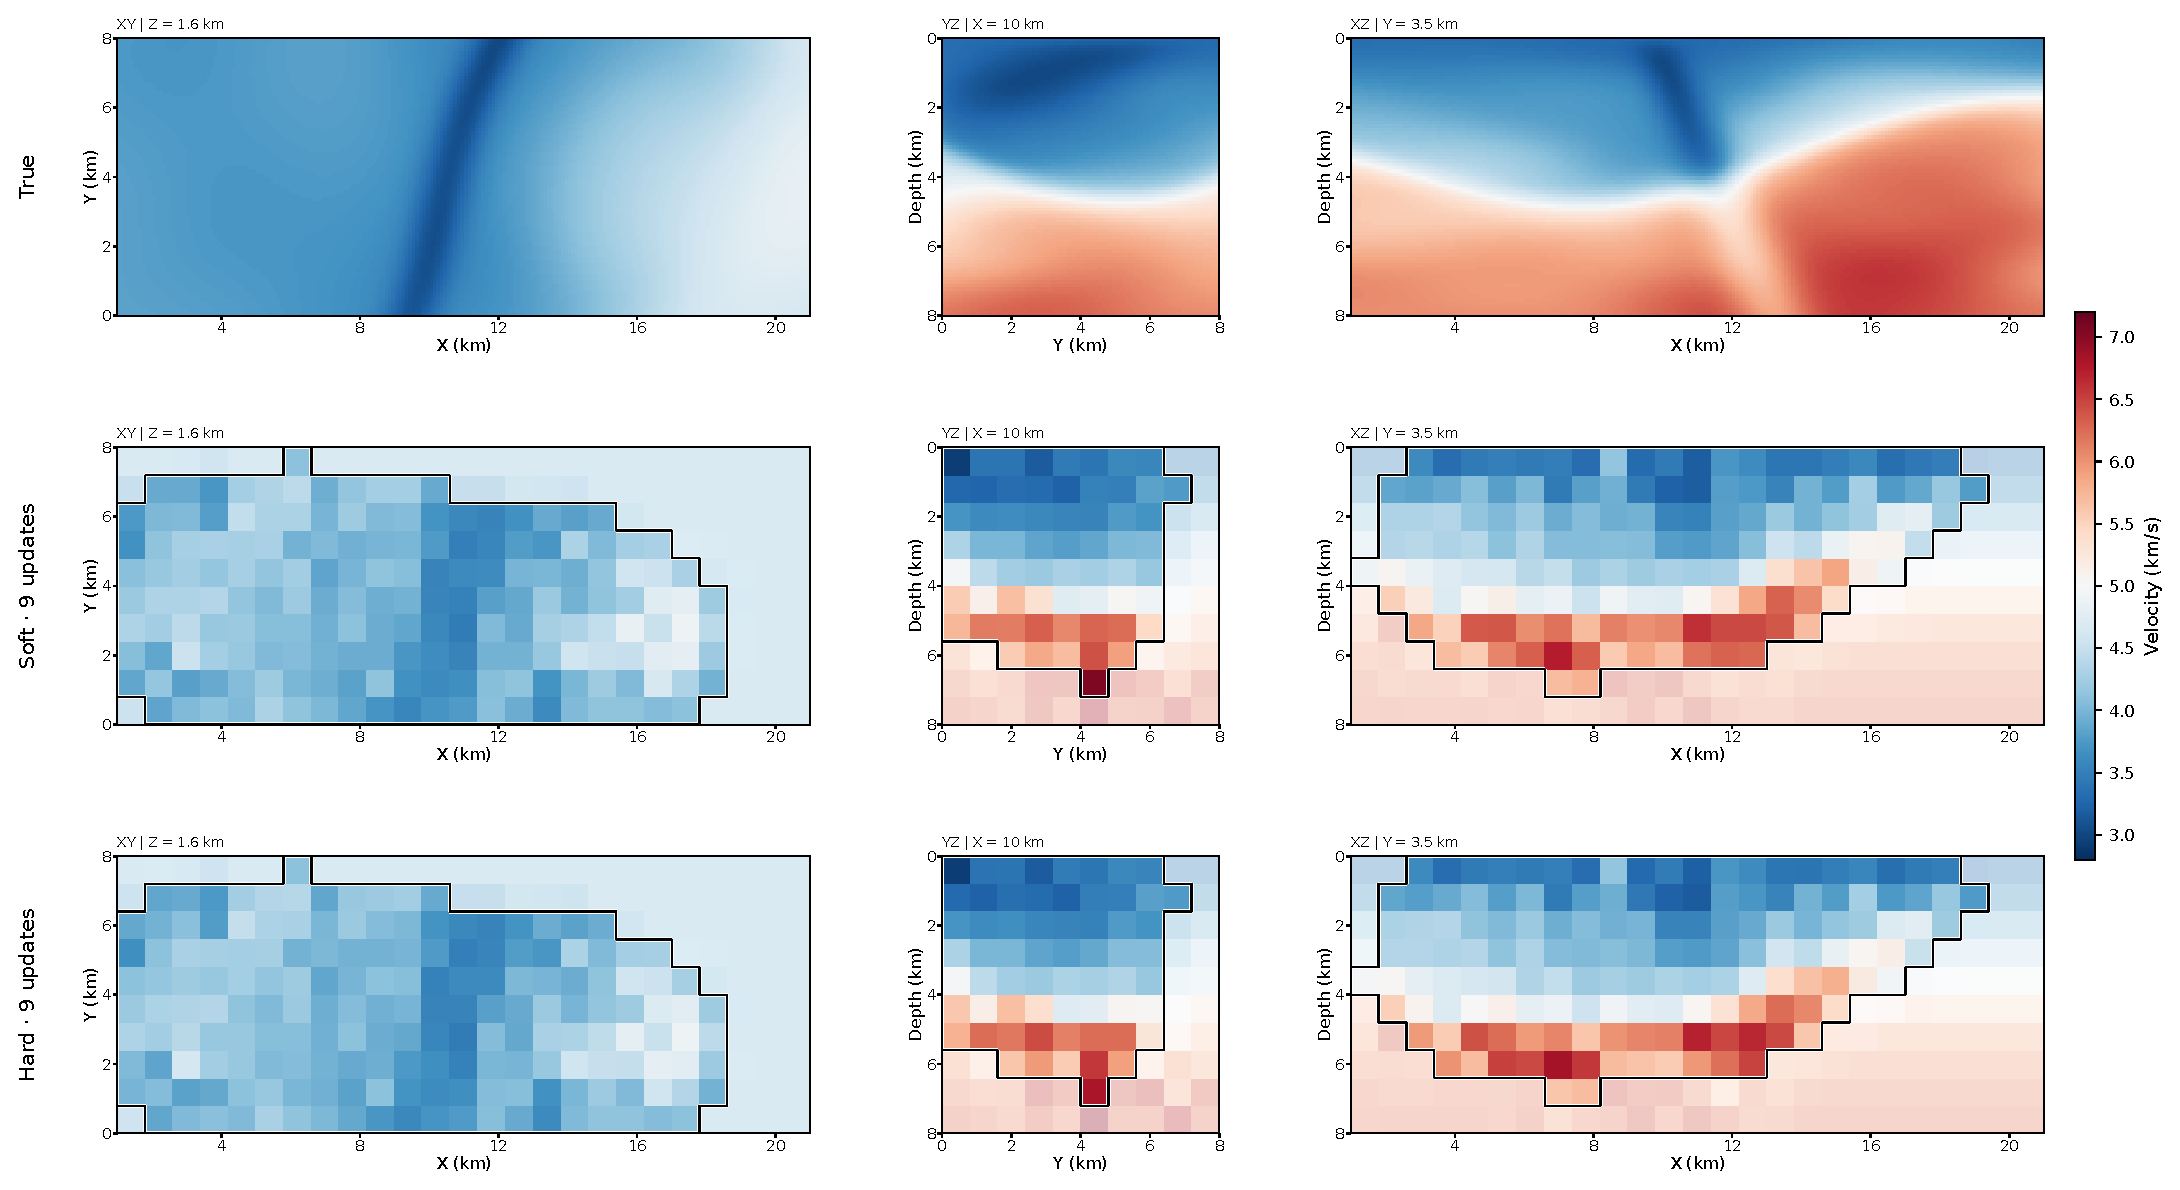
\includegraphics[width=\textwidth,height=0.63\textheight,keepaspectratio]{figures/used/section_4_6_final.pdf}
\begin{singlespace}
\caption{Heterogeneous model: truth, final soft reconstruction, and final hard reconstruction (top to bottom), using the favorable truth-informed 1-D start. Both reconstructions have nine updates and correspond to the 1-D rows of Table~\ref{tab:heterogeneous_comparison}. Columns show $XY$ at $Z=1.6$~km, $YZ$ at $X=10$~km, and $XZ$ at $Y=3.5$~km in the fault-test frame; native $X$ coordinates are shifted by $+1$~km. The common hard/soft sensitivity envelope follows Figure~\ref{fig:fault_sections_final}, here on 800-m cells with one-cell expansion. Fading denotes the outside of this display envelope, not demonstrated lack of resolution; the envelope itself does not establish good resolution. Diagnostics precede the final update, and the velocities retain their native piecewise-constant cells without smoothing.}
\label{fig:heterogeneous_sections_final}
\end{singlespace}
\end{figure}
\FloatBarrier

\subsection{Real Data}
\label{subsec:real_data_results}

We apply hard and soft EMTomo to P-wave arrival picks from The Geysers geothermal field, California, recorded on 1--20 April 2011. Picks come from the NCEDC EGS/BG catalog, with station metadata from its FDSN Station service \parencite{ncedc2014}. After requiring at least six available picks per event, the retained data comprise 47,748 picks from 3471 events at 31 stations. We preserve missing observations and add no synthetic noise. Both inversions begin with the same linear $V_P$ profile, increasing from 3.5 to 6.0~km/s across the 7-km model depth, on 1-km velocity cells. Each then continues from its own recovered model on 500-m cells, keeping the travel-time grid at 125~m. We compare the recovered velocity structures with the published 3-D $V_P$ model of \textcite{guo2021geysers}, available in their model archive \parencite{guo2021geysersdata}. Their tomography uses a different, partly overlapping 2011 event set, repicked P arrivals, and catalogue and waveform differential times. 

We evaluate the final models selected by internal-control stopping. The prediction protocol in Section~\ref{subsec:metrics} uses 38,676 training picks and scores 4775 external held-out picks from 3186 events. The common location search uses 50 candidates, 875-m seed separation, and likelihood standard deviations of 1\% relative, 0.05~s absolute, and 0.02~s model uncertainty. The 4297 internal control picks remain excluded from location fitting. The external split was inspected for earlier models, so it is not an untouched test set. Structural comparison is restricted to published coverage with scaled resolvability above 0.4, corresponding to the outlined, unfaded regions in Figure~\ref{fig:real_picks_sections_final}. Model differences are sampled at 125-m spacing.

% Metrics: exp_data/geysers_real_holdout_latest/summary.json;
% exp_data/geysers_real_structure_comparison.json; exp_data/geysers_real_location_shifts_latest.json.
\begin{figure}[!htbp]
\centering
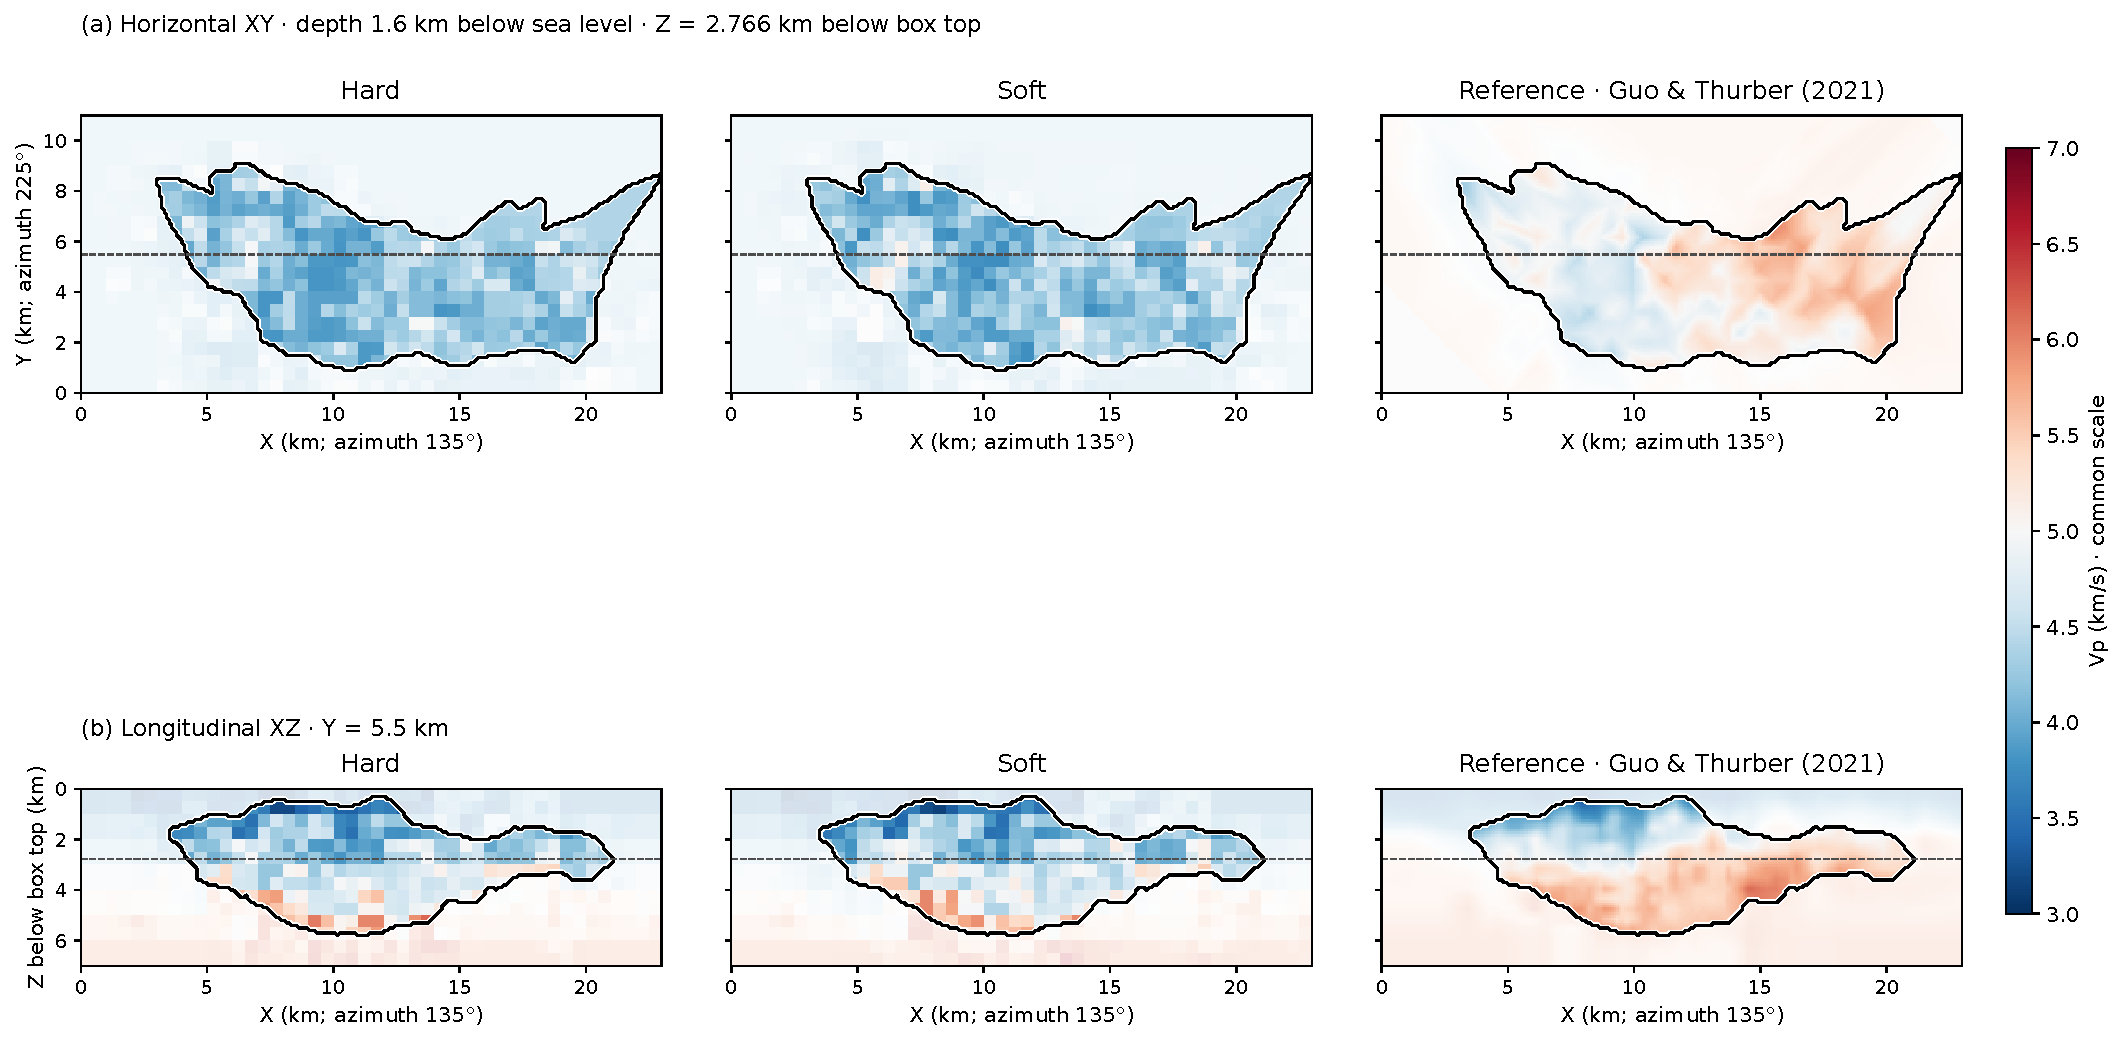
\includegraphics[width=\textwidth]{figures/used/real_picks_comparison_final.pdf}
\begin{singlespace}
\caption{The Geysers real-pick velocity models: final hard and soft EMTomo reconstructions and the published reference of \textcite{guo2021geysers}. Top: horizontal section at 1.6~km below sea level ($Z=2.766$~km below the model top); bottom: vertical section at $Y=5.5$~km. Dashed lines mark the other section's trace. Black outlines enclose reference coverage with published scaled resolvability $R>0.4$; the same mask and outside fading are applied to all models. This reference-derived region does not establish hard/soft resolution, and the published model is not ground truth. Hard/soft velocities retain native, unsmoothed 500-m cells; 100-m plotting samples do not imply 100-m resolution.}
\label{fig:real_picks_sections_final}
\end{singlespace}
\end{figure}
\FloatBarrier

Held-out arrival-time RMSE decreases from 105.92~ms for the initial model to 96.73~ms for hard and 95.73~ms for soft, reductions of 8.67\% and 9.62\%. Soft improves on hard by 1.04\%, but the 95\% interval from 2000 paired event-bootstrap samples spans $-0.72$ to $2.55\%$, so the difference remains uncertain on this split. Within the resolved part of the published model, RMS velocity differences are 0.617, 0.730, and 0.735~km/s for initial, hard, and soft, respectively. Better pick prediction therefore does not imply closer agreement with that reconstruction. Both relocations tend to move events deeper than the catalog, with median signed depth shifts of 113~m for hard and 202~m for soft. Their median pairwise 3-D separation is 145~m.
